%
%%%%%%%%%%%%%%%%%%%%%%%%%%%%%%%%%%%%%%%%%%%%%%%%%%%%%%%%%%%%%%%%%%%%%%%%%%%%%%%
% The LHC
%%%%%%%%%%%%%%%%%%%%%%%%%%%%%%%%%%%%%%%%%%%%%%%%%%%%%%%%%%%%%%%%%%%%%%%%%%%%%%%
%
\chapter{The ATLAS detector at the LHC}

\section{The Large Hadron Collider}


The Large Hadron Collider  (LHC)~\cite{Breskin:1244506} is a proton-proton ($pp$) synchrotron located in the previous Large Electron Positron (LEP) collider tunnel at CERN Laboratory, just outside the city of Geneva (Switzerland), approximately 100~m underground. It is designed to collide bunches of up to $\sim 10^{11}$ protons every 25~ns at a center-of-mass energy of 14~TeV (seven times the 2~TeV reached by the Tevatron accelerator at Fermilab Laboratory, in Chicago). 

The experiments analyzing the collisions produced by the LHC are distributed around the 27~km ring at the various interaction points. The ATLAS experiment is located at Point 1, which is closest to the main CERN site. Point 5 houses the other general purpose detector, CMS. ALICE and LHCb experiments are located at Point 2 and Point 8, respectively. The former is designed to investigate heavy ion collisions; the latter, to investigate rare decays of b-mesons. The layout of these four experiments along the LHC ring is shown in Fig.~\ref{fig:LHC1}.

\begin{figure}[htbp]
  \begin{center}
      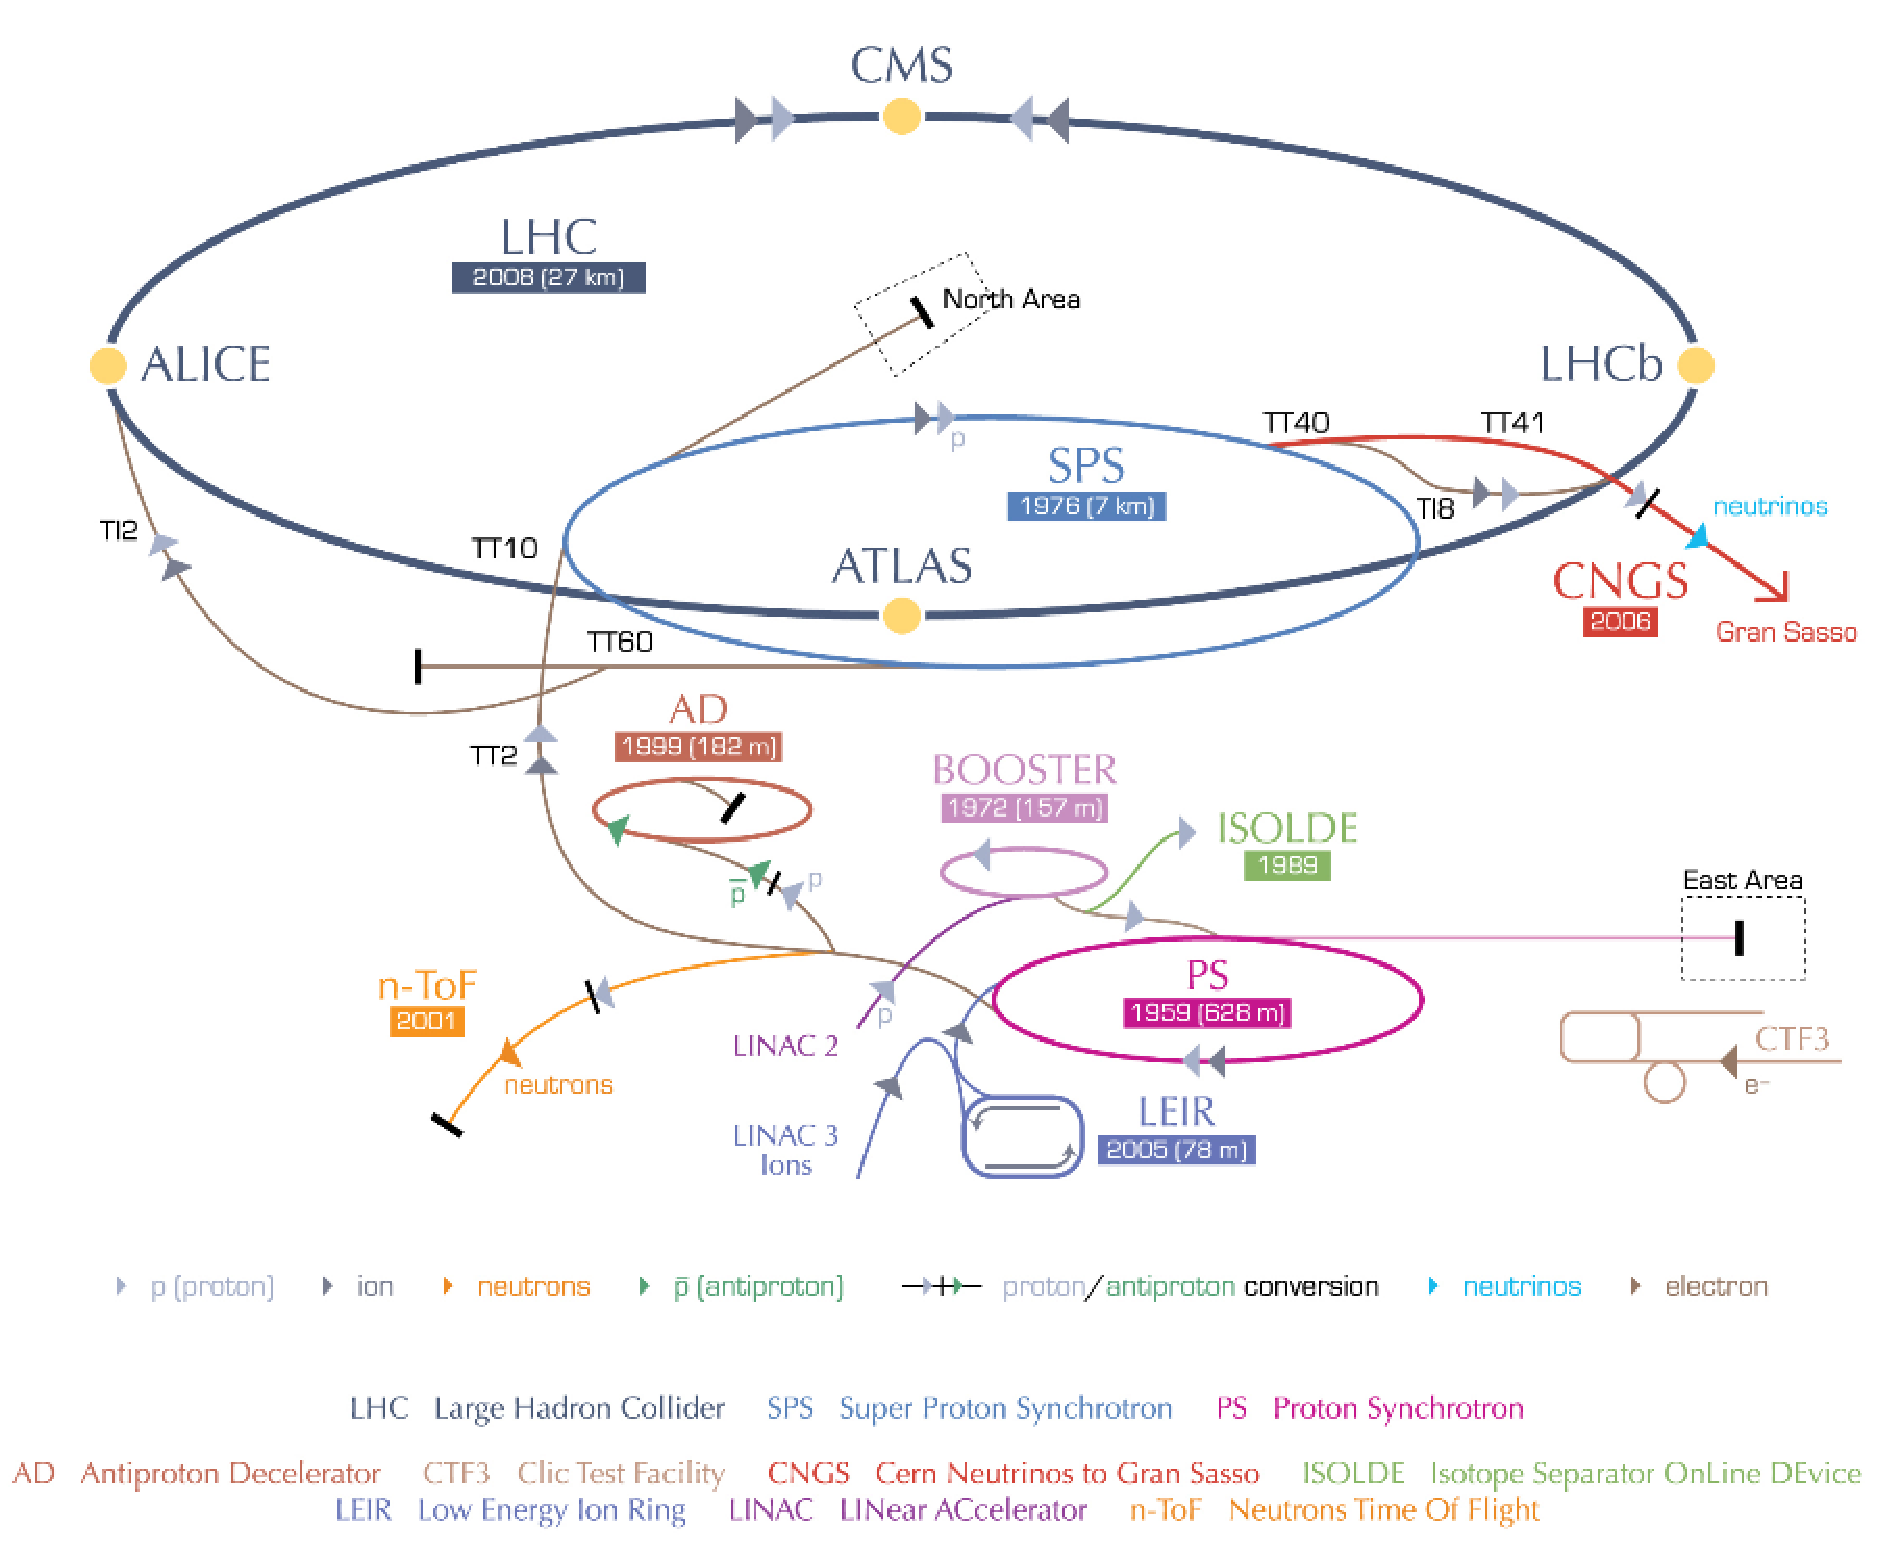
\includegraphics[width=1\textwidth]{Fig2/CERNacceleratorcomplexCut.pdf}
    \caption{The CERN accelerator complex, showing the injection system, along with each component’s date of construction, and the placement of the four main experiments.}
    \label{fig:LHC1}
  \end{center}
\end{figure}


Proton beams are formed, before insertion into the main LHC ring, using a succession of smaller machines with increasingly  higher energies, as shown in Fig.~\ref{fig:LHC1}. The chain begins as protons are injected into the PS Booster (PSB) at an energy of 50~MeV from Linac2. The booster accelerates them to 1.4~GeV. The beam is then fed to the Proton Synchroton (PS) where it is accelerated to 25~GeV. At desin strength, the bunch structure, known as a bunch train, contains 72 bunches of protons upon entry to the Super Proton Synchrotron (SPS). The SPS accumulates up to four fills of 72 bunches from the PS and accelerates them to 450~GeV, with a bunch spacing of $\sim$~25~ns. They are finally transferred to the LHC (both in a clockwise and an anticlockwise direction) where they are accelerated for 20 minutes to their nominal energy of 7 TeV. Beams will circulate for many hours inside the LHC beam pipes under normal operating conditions.

The bunch structure is a direct consequence of a radio frequency (RF) acceleration scheme used to attain the desired high proton beam energy.  In RF acceleration, particles travel through a series of time-varying electrical fields and they can only be accelerated when the RF field has the correct orientation when particles pass through an accelerating cavity, which happens at well specified moments during an RF cycle. The result of a sequence of RF accelerations is several bunches of protons. It is important to note that when we speak about ``beams'' we refer to many bunches of protons separated by some uniform distance. Increasing the number of bunches is one of the ways to increase luminosity in a machine (more about luminosity in subsection~\ref{sec:lumiintro}). At desinged beam intensitity, when the bunches cross, there will be a maximum of about 20 collisions.

A larged magnetic field is needed to guide and maintain the beam particles in their circular orbit. The needed field is achieved using superconducting electromagnets built from NbTi coils that operate in a superconducting state, efficiently conducting electricity without resistance or loss of energy. The currents through the coils produce magnetic fiedls perpendicular to the direction of motion of the protons that deflect the protons into their orbits.  The whole magnetic system comprises 1232 dipole magnets of 15~m length which are used to bend the beams, and 392 quadrupole magnets, each 5–7~m long, to focus the beams. At a peak beam energy of 7~TeV, the dipoles need to produce an 8.33~T magnetic field, requiring a current of $\sim$ 12~kA. In order to deliver the current densities and magnetic field required for 7~TeV proton beams, the magnets are kept at 1.9~K by circulating superfluid helium.

The first $pp$ collisions produced by the LHC ocurred on November 23 2009, at the SPS extraction energy of 450~GeV per beam. Very quick after, on December 8, ATLAS and CMS detectors started recording data at energy of 2.36~TeV. By this time the LHC became the highest energy accelerator in the world.  During this period, bunch intensities were limited by machine-protection considerations to 1.5 $\times$ 10$^{10}$ protons.

 In February 2010, the LHC was commissioned once more with 450 GeV beams, and a series of tests were performed to ensure that the magnet systems could operate safely at the currents necessary to control 3.5 TeV beams. This was followed by the very first collisions at 7~TeV center-of-mass energy on March 30. During the 2010 run the beam parameters were tuned (the beam widths squeezed and the number of protons per bunch and the number of bunches in each beam increased) in order to increase the beam intensity.  In particular, as the intensity of the beams increased, the mean number of interactions per bunch crossing increased.  


Finally, the data samples analysed in this thesis correspond to proton-proton collisions at $\sqrt{s}=7$ TeV delivered by the LHC and recorded by ATLAS between May and November 2011, with the LHC running with 50~ns bunch spacing. Table~\ref{tab:beamparameters} summarizes the basic beam parameters expected for design energy and luminosity and the beam parameters as of May 2011. The LHC performance steadily improved during 2011. The average number of interactions per bunch crossing throughout the data-taking period considered rapidly increased approximately from $\sim$3 to 8 until (northern hemisphere) summer 2011, with a global average for this period of $\approx 6$. Starting in August 2011 and lasting through the end of the proton run, this number ranged from approximately 5 to 17, with an average of about 12. This evolution is illustrated in Fig.~\ref{fig:peakAvgMu}, which shows the maximum mean number of collisions per beam crossing versus day in 2011. 


\begin{table}[!hbt] %[h]
\renewcommand{\arraystretch}{1.2}
\centering
\begin{tabular}{ | c | c | c |}
\hline
  ~~~~~~~~~~~~~~~~Parameter~~~~~~~~~~~~~~~~ &~~~~~~2011 runs~~~~~~ &~~Design~~ \\ \hline
  Center-of-mass energy [TeV]         &  7    & 14 \\ 
  Instantaneus luminosity [cm$^{-2}$s$^{-1}$]     & 3.65 10$^{33}$ (year peak)  & 10$^{34}$     \\ 
  Bunches per beam  &  38 (May)  & 2808        \\ 
  Protons per bunch &  0.8$\times$10$^{11}$ (May)   & 1.5$\times$10$^{11}$    \\
  Mean interactions per crossing  &  6 to 12 (year average) & 23        \\ \hline 
\end{tabular}
\caption{Summary of beam conditions during the 2011 7 TeV runs and those foreseen at design energy and luminosity.
}
\label{tb:beamparameters}
\end{table}


\begin{figure}[htbp]
  \begin{center}
      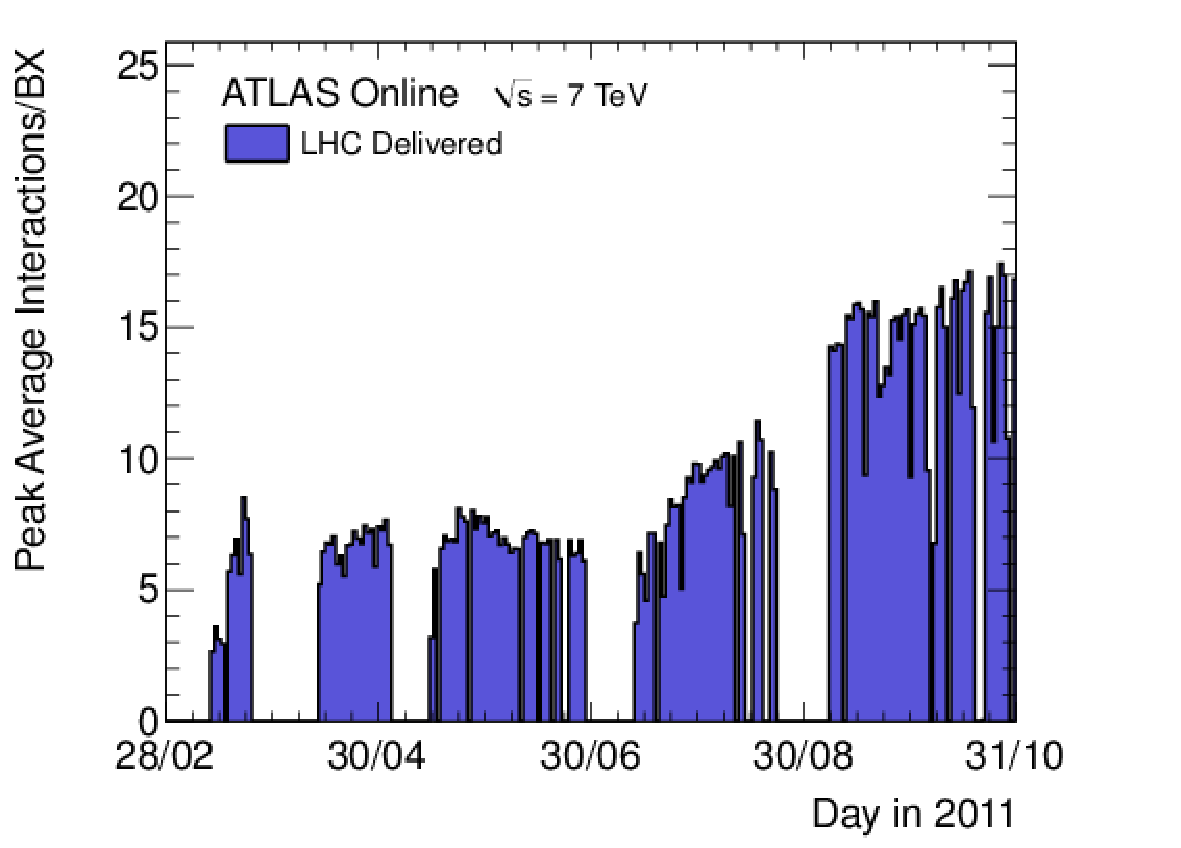
\includegraphics[width=0.7\textwidth]{Fig2/peakAvgMuByDay.pdf}
    \caption{The maximum mean number of events per beam crossing versus day in 2011.}
    \label{fig:peakAvgMu}
  \end{center}
\end{figure}


%------------------------------------------------------------------------
\subsection{Luminosity and pile-up}\label{sec:lumiintro}
%------------------------------------------------------------------------

The rate of events produced by the colliding beams depends on the luminosity of the collisions, which is a measure of the number of events per second per unit cross section, typically measured in units cm$^2$s$^{-1}$. The number of events of a particular process, then, is given by the product of the integrated luminosity, $\int dt L$, and the cross section of the process, $\sigma_{event}$.  The integrated luminosities are typically quoted in units of inverse picobarns, pb$^{-1}$~=~10$^{-36}$cm$^{2}$. In order to measure processes with very little cross sections a very high luminosity is required. 

The delivered luminosity can be written as~\cite{ATLAS-CONF-2011-116}:

\begin{equation} 
\mbox{ {\it L }} = \frac{n_b f_r n_1 n_2 }{2\pi \Sigma_x \Sigma_y}
\label{eqn:lumi}
\end{equation} 
where n$_b$ is the number of colliding bunch pairs,  n$_1$ and n$_2$ are the bunch populations (protons per bunch) in beam 1 and beam 2 respectively (together forming the bunch charged product), $f_r$ is the machine revolution frequency, and $\Sigma_x$ and $\Sigma_y$ are the width and the height of the proton beams. %characterize the horizontal and vertical profiles of the colliding beams. 

The number of protons per bunch, the number of bunches per beam, and the revolution frequency are all set by the beam operators. The widths of the proton beams are measured in a process known as a Van der Meer ($vdM$) scan~\cite{vanderMeer:296752}. In a $vdM$ scan, the beams are separated by steps of a known distance. The collision rate is measured as a function of this separation, and the width of a gaussian fit to the distributions yields the width of the beams in the direction of the separation.  

The total integrated luminosities provided by the LHC and recorded by ATLAS in 2011 are shown in Figure~\ref{fig:integratedlumi}. These events form the dataset analyzed in this thesis. By means of the beam-separation or $vdM$ scans, as well as other techniques to measure the bunch charged product, the ATLAS Collaboration has determined that the uncertainty on its luminosity measurement is $\delta L = \pm 3.7$\%. For a complete description of the methods used and the systematic erros evaluated see reference~\cite{ATLAS-CONF-2011-116}.

\begin{figure}[htbp]
  \begin{center}
      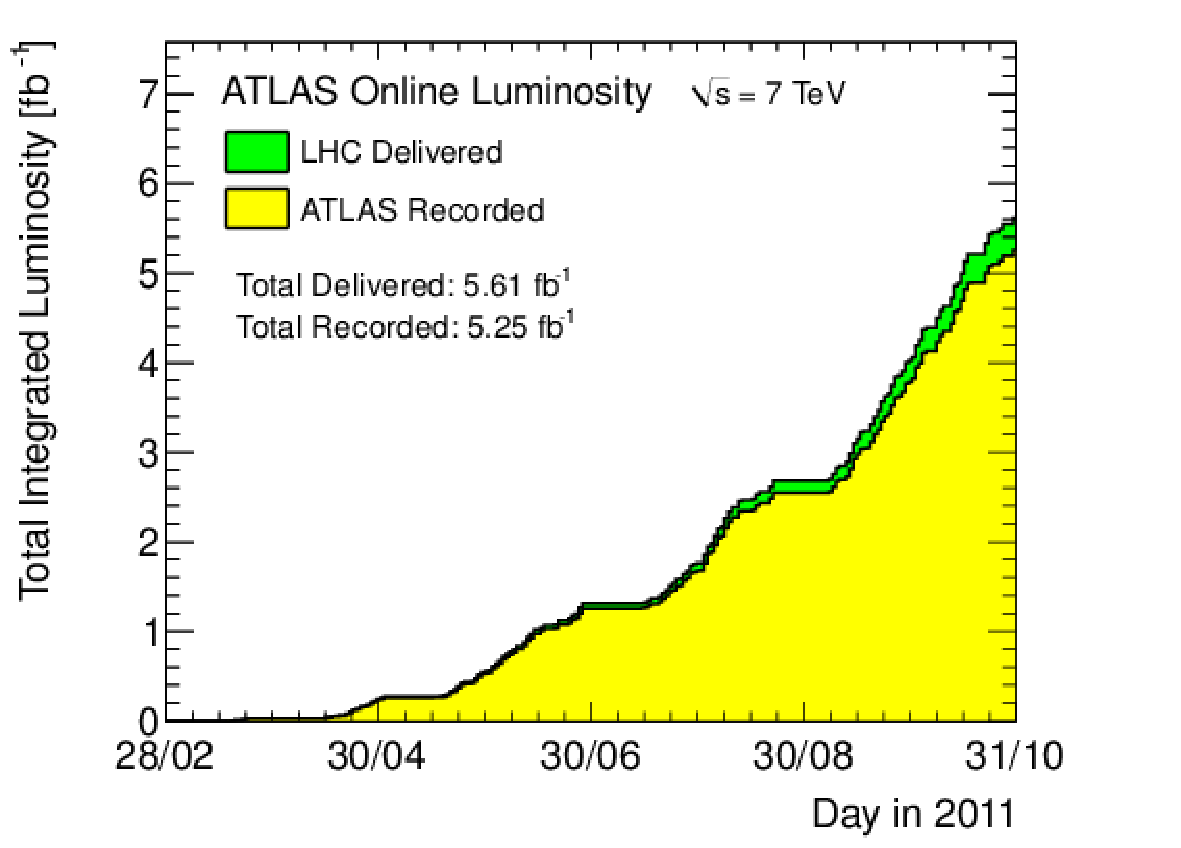
\includegraphics[width=0.7\textwidth]{Fig2/sumLumiByDay.pdf}
    \caption{Total luminosity delivered by the LHC and recorded by ATLAS during the 2011 $sqrt{s}$ = 7~TeV proton-proton run}
    \label{fig:integratedlumi}
  \end{center}
\end{figure}


As anticipated, due to the cross-section for interaction and the number of protons per bunch, the possibility to observe multiple $pp$ interactions per bunch crossing increases proportionally. This phenomenon, referred to as ``pile-up'', can really occur in two distinct forms. The first form is the presence of multiple $pp$ collisions (different from the interaction of interest) in the same bunch crossing, referred to as ``in-time'' pile-up. The second form of pile-up takes place due to electronic integration times within the detector. Certain detector components are actually sensitive to multiple bunch crossings due to the long electronic signals generated in the response to energy depositions or charge collection. One or more $pp$ collisions in a bunch-crossing different from that which produced the collision of interest can then affect the measurement. This form of pile-up is referred to as ``out-of-time'' pile-up and will become more and more important as the LHC bunch spacing gets closer to the nominal value, 25~ns.

The fraction of events with pile-up increased significatively since the data taking started. The experimental signature of this fact is obtain via the number of reconstructed primary vertices, or NPV. The effect of the event NPV is an important concern for the measurement of jet properties and will be discussed in the next chapters.


%
%%%%%%%%%%%%%%%%%%%%%%%%%%%%%%%%%%%%%%%%%%%%%%%%%%%%%%%%%%%%%%%%%%%%%%%%%%%%%%%
% ATLAS
%%%%%%%%%%%%%%%%%%%%%%%%%%%%%%%%%%%%%%%%%%%%%%%%%%%%%%%%%%%%%%%%%%%%%%%%%%%%%%%
%
\section{The ATLAS Detector}

%------------------------------------------------------------------------
%\subsection{Detector overview}\label{sec:atlassummary}
%------------------------------------------------------------------------

The ATLAS detector~\cite{ATLAS} is one of the two general purpose particle detectors built for probing $pp$ collisions at the LHC. As it was described in the previous section, inside the LHC, bunches of up to 10$^{11}$ protons will collide 40 million times per second to provide 14~TeV proton-proton collisions at a nominal luminosity of 10$^{34}$cm$^{-2}$s$^{-1}$. These high interaction rates and energies, as well as the requirements for high precision physics measurements set the standars for the design of the detector. At even 7 TeV center-of-mass energy, the LHC interactions result in high particle multiplicity, requiring fine detector granularity, and particle production at forward rapidity, requiring large detector angular coverage.

To achieve these performance goals, a design consisting of multiple detector sub-systems with cylindrical symmetry around the incoming beams is used as shown in Fig.~\ref{fig:ATLAS}. Closest to the interaction point the inner tracking detector is placed, providing charged particle reconstruction. The magnet configuration comprises a thin superconducting solenoid surrounding the inner detector cavity, and three large superconducting toroids (one barrel and two end-caps) arranged with an eight-fold azimuthal symmetry around the calorimeters. This fundamental choice has driven the design and size (44~m in length and 25~m in height) of the rest of the detector. Outside the solenoid, a calorimeter system performs electron, photon, tau, and jet energy measurements. Finally, the calorimeter is surrounded by the muon spectrometer where an array of muon drift chambers perform muon identification and momentum measurements.

The ATLAS detector coordinate system is used to describe the position of particles as they traverse these subdetectors. It is a right-handed coordinate system, with z pointing along the beam direction, positive x pointing toward the center of the LHC ring, and positive y pointing up. The x − y plane is referred to as the transverse plane, and the z direction as the longitudinal
direction. The azimuthal angle $\phi$ is measured as usual around the beam axis, and the polar angle $\theta$ is the angle from the beam axis. The pseudorapidity is defined as $\eta = − ln tan(\frac{\theta}{2})$, regions of low $\eta$ are referred to as ``central'', and regions of high $\eta$ are referred to as ``forward''. % (in the case of massive objects such as jets, the rapidity y = 1/2ln[(E + pz )/(E − pz )] is used). 
The transverse momentum $\pt$ is defined in the x-y plane unless stated otherwise. The distance $\Delta R$ in the pseudorapidity-azimuthal angle space is defined as $Delta R = \sqrt{ \Delta \eta^2  + \Delta \phi^2}$ .

\begin{figure}[htbp]
  \begin{center}
      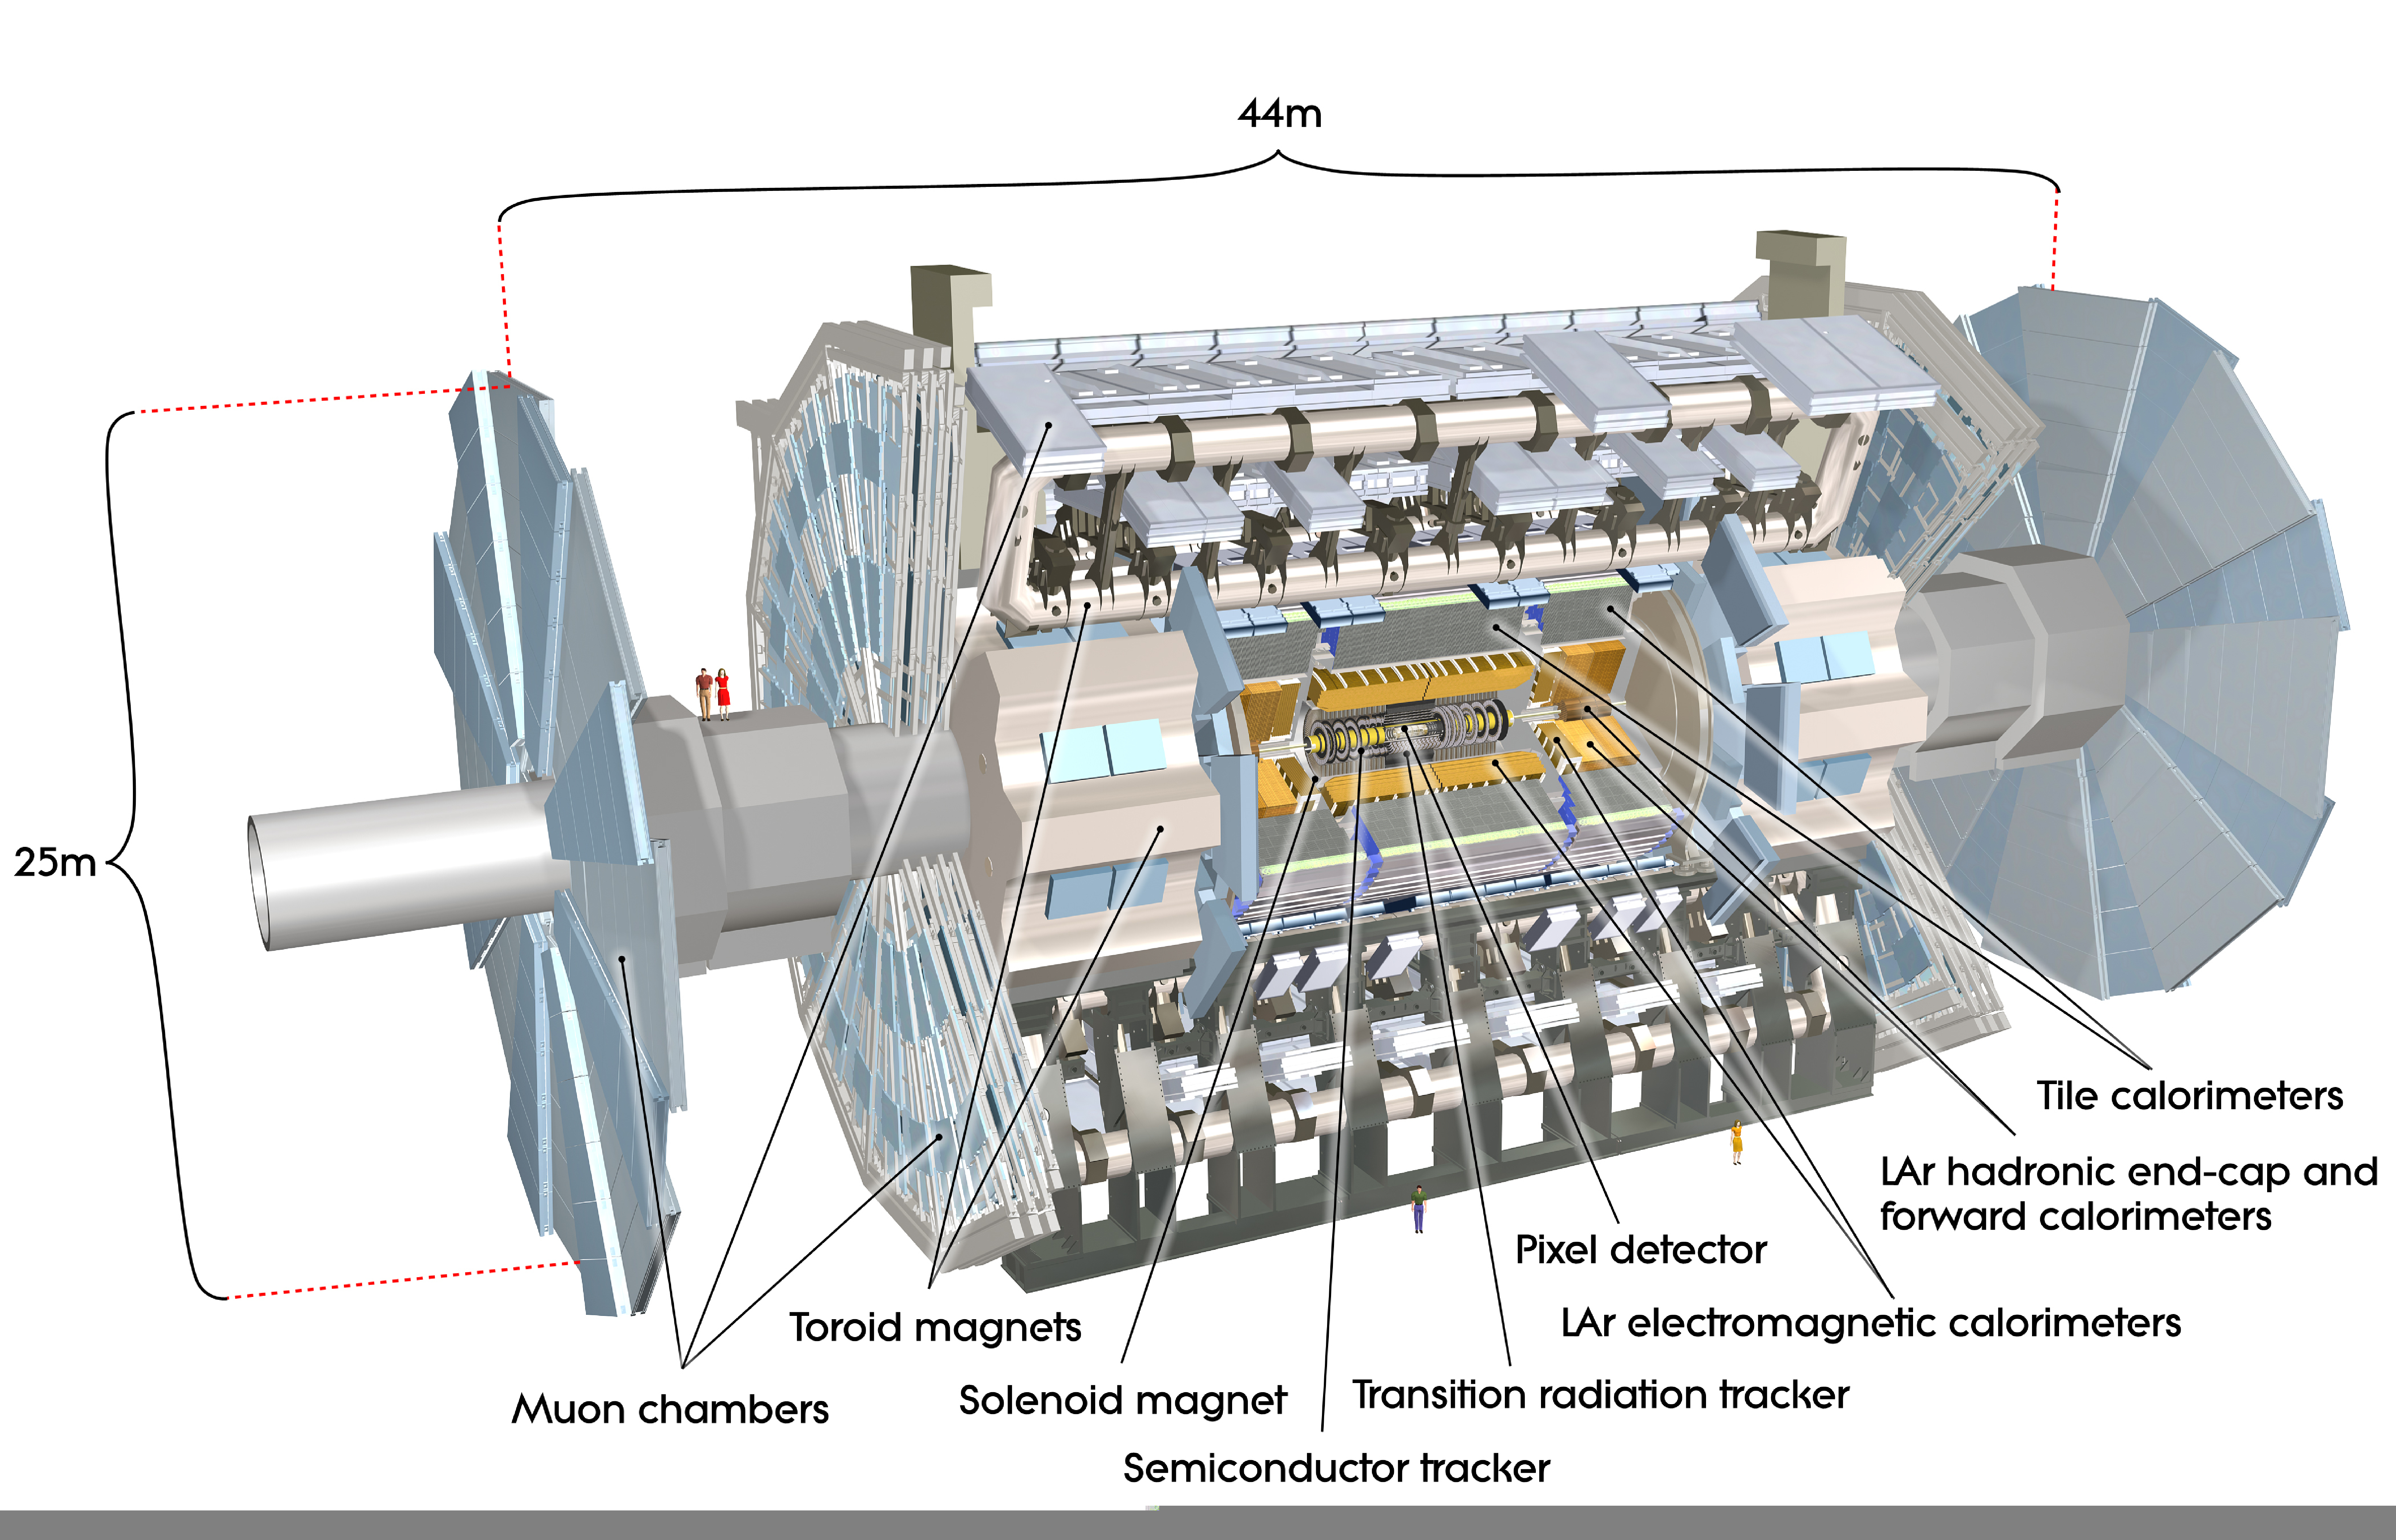
\includegraphics[width=0.9\textwidth]{Fig2/ATLASDetector.pdf}
    \caption{El detector de ATLAS}
    \label{fig:ATLAS}
  \end{center}
\end{figure}

To meet the extremely high demands that the LHC luminosity places on the speed with which ATLAS must record data, a dedicated trigger and data acquisition (TDAQ) systema is used. The interaction rate at the design luminosity is approximately 1~GHz, while the event data recording, based on technology and resource limitations, is limited to about$\sim$200~Hz. This requires a high rejection of minimum-bias processes while maintaining maximum efficiency for the new physics. The Level-1 (L1) trigger system uses a
subset of the total detector information to make a decision on whether or not to continue processing an event, reducing the data rate to approximately 75~kHz (limited by the bandwidth of the readout system, which is upgradeable to~100 kHz). The subsequent two levels, collectively known as the high-level trigger (HLT), are the Level-2 (L2) trigger and the event filter. They provide the reduction to a final data-taking rate of approximately 200 Hz. 



%------------------------------------------------------------------------
\subsection{Inner tracking system}\label{sec:atlasID}
%------------------------------------------------------------------------

The inner tracking system or inner detector (ID) is composed of three subdetectors: the pixel detector, the semiconductor tracker (SCT) and the transition radiation tracker (TRT). The goal of these three is to provide charged particle trajectory reconstruction and momentum measurements with an overall acceptance in pseudorapidity of $|\eta| < 2.5$ and full $\phi$ coverage. 

The sensors which built this system register signals, referred to as ``hits'', in response to the passage of charged particles. The ID is inmersed in a 2~T magnetic field, generated by the central solenoid. The positions of the registered hits are combined to form tracks, with the radius of curvature  of the tracks (caused by the presence of the magnetic field) providing a measurement of the particle’s transverse momentum. The track reconstruction efficiency ranges from 78\% at $p^{track}_{T} = 500$~MeV to more than 85\% above 10~GeV, averaged across the full $\eta$ coverage~\cite{chargemultiplicity}. The transverse momentum resolution of $\sigma_{p_T}$/$\pt$ = 0.05~\cite{ATLAS-CONF-2010-009} (upper bound) and a transverse impact parameter resolution of $\sim$20~ $\mu m$ for high momentum resolution particles in the central $\eta$ region\cite{ATLAS-CONF-2010-070}. 

The pixel detector, SCT, and TRT sensors are arranged on concentric cylinders around the beam axis, known as barrel layers, and on disks perpindicular to the beam at either end of the barrel, known as end-caps. A more complete description of these systems is given below. The overall layout of the inner detector is shown in Fig.~\ref{fig:figinner}. 


\begin{figure}[htbp]
  \begin{center}
      \includegraphics[width=0.9\textwidth]{Fig2/InnerDetector.pdf}
    \caption{Layout of the ATLAS inner detector.}
    \label{fig:figinner}
  \end{center}
\end{figure}


\subsubsection{The Pixel detector}

The pixel detector consists of three concentric barrel layers. The innermost one, the so called ``b-layer'' due to its role in identifying $b$-quarks initiated jets, is located at 5~cm from the interaction region. Three additional disks are located at each end-cap, producing typically three pixel position measurements per charged particle track.  Each layer or disk is instrumented with modules that form the basic unit of data acquisition, each with 47232 pixels.  All pixel sensors are identical and have a minimum pixel size in $r$ - $\phi \times z$ of 50 $\times$ 400~$\mu m^2$. The intrinsic accuracies in the barrel are 10 $\mu m$ in $r$ - $\phi$ and 115 $\mu m$ along $z$, or along $r$ in the end-caps. The pixel detector has approximately 80.4 million readout channels, an order of magnitude more readout channels than the rest of ATLAS combined, and it extends to a total length of $z \sim \pm$650~mm and radius of $r \sim$150~mm, providing good reconstruction efficiency for tracks up to $|\eta| <$2.5.

 
\subsubsection{The SCT}


The SCT consists of four barrel layers and nine end-cap layers surrounding the pixel detector, resulting in at least four hits along every charged particle track.  The SCT barrel reaches to $z\sim \pm$750~mm and $r \sim $515~mm, while the end-cap covers out to $z\sim \pm$2720~mm and $r =$560~mm.  There are 15,912 SCT module sensors, each 12.8~cm long and approximately 285~$\mu $m thick. 

In the barrel region, these modules use small-angle (40~mrad) stereo strips to measure both coordinates, with one set of strips in each layer parallel to the beam direction, measuring the $\phi$ coordinate directly . In the end-cap region, the detectors have a set of strips running radially and a set of stereo strips at an angle of 40~mrad. The mean pitch of the strips is 80~$\mu m$. The intrinsic accuracies per module in the barrel are 17~$\mu m$ in $r$ - $\phi $ and 580~$\mu m$ in $z$ (or $r$ in the end-caps). The total number of readout channels in the SCT is approximately 6.3 million.  A hit is registered only if the pulse height in a channel exceeds a preset threshold ($\sim $ 1~fC). The charged measured in the strip is then recorded into a memory buffer that is only read out and used for tracking if a trigger is received signaling that the event should be considered in more detail.


  
\subsubsection{The TRT}

The TRT surrounds the silicom detectors and is comprised of up to 76 layers of longitudinal straw tubes in the barrel, extending to $z\sim \pm$710~mm and $r \sim$1060~mm, and 160 radial straw planes in each end-cap cylinders, reaching $z\sim \pm$2710~mm and $r \sim$1000~mm.

 The TRT sensors are thin drift tubes consisting of cathode metal straws filled with an ionizing gas mixture of xenon, oxygen, and CO$_2$, with an anode wire running down the center of the straw. The passage of a charged particle through the gas produces positive ions and free electrons, which travel to the cathode and anode, respectively, under the influence of an applied voltage of 1600~V. Comparing the time that the signals are received at the cathode and the anode gives a drift time measurement that can be used to calculate the impact parameter of the particle. This method gives no information on the position along the length of the straw.

To give the best resolution of particle trajectories as they bend in the solenoidal field, the straws lie along the beam direction in the barrel and radially in the end-caps. The straw diameter of 4~mm causes a maximum drift time of approximately 48~ns and an intrinsic accuracy of 130 μm along the radius of the straw.

In addition to directly detecting charged particles produced by the collision, the TRT also measures the transition radiation induced by the passage of these particles through polypropylene sheets placed between the drift tube straws. Transition radiation refers to the photons emitted by charged particles as they pass from one material into another with a different dielectric constant. These photons yield a much larger signal amplitude than the charged particles, so separate thresholds in the electronics can be used to distinguish the two.

 
 % Este sistema de detecci\'on por tubos provee un gran n\'umero de puntos por traza (t\'ipicamente 36 puntos), lo cual determina un seguimiento cont\'inuo de la misma, con mucho menos material por punto y menor costo (mucho menor comparado con la tecnolog\'ia de p\'ixeles implementada en el subdetector m\'as interno).  La gran cantidad de puntos o impactos por traza es un instrumento poderoso en la b\'usqueda y reconstrucci\'on de trazas en el detector interno.

One of the most important tasks of the inner detector is to provide accurate collision vertex identification, exploiting the excellent position resolution and tracking efficiency. Vertices are reconstructed by matching inner detector tracks with $\pt >$ 150~MeV back to a common origin.% [67].

%------------------------------------------------------------------------
\subsection{The Calorimeter System}\label{sec:atlasCALO}
%------------------------------------------------------------------------

The purpose of the ATLAS calorimeter system is to measure the energy of electrons, photons, taus and jets, within the pseudorapidity region of $|\eta| < $4.9 and with full $\phi$ symmetry and coverage around the beam axis. It also provides fast position and energy measurements to serve as trigger signals for these objects as well as the missing transverse energy. 

The calorimeter detector consist of electromagnetic (EM) calorimeter and hadronic calorimeter components. The EM calorimter provides fine granularity measurements of electrons and photons.  Each calorimeter is segmented both transverse to the particle direction, to give position information, and along the particle direction, to chart the development of the particle shower.  This permits detailed mapping of EM and  hadronic showers in the calorimeter, allowing for studies of the internal structure of hadronic jets and partially giving rise to the high resolution measurements of their energy.
%%%%%provides detailed information on the transverse and longitudinal shower shapes of hadronic jets.

%It consists of an electromagnetic (EM) calorimeter covering the pseudorapidity region $|\eta| < 3.2$, a hadronic barrel calorimeter covering $|\eta| < 1.7$, hadronic end–cap calorimeters covering $1.5 < |\eta| < 3.2$, and forward calorimeters covering $3.1 < |\eta| < 4.9$. 
The EM and hadronic calorimeters are sampling calorimeters meaning that they utilize alternating layers of absorber material, composed of heavy atoms that interact with energetic particles and cause them to loose energy, and an active material, that produce a signal in response to the deposited  energy.

The calorimeters closest to the beam-line are housed in three cryostats, one barrel and two end-caps. The barrel cryostat contains the electromagnetic barrel calorimeter, and the two end-cap cryostats each contain an electromagnetic end-cap calorimeter (EMEC), a hadronic end-cap calorimeter (HEC), located behind the EMEC, and a forward calorimeter (FCal) to cover the region closest to the beam.  These calorimeters use liquid argon as the active detector medium and need to be mantained at a constant temperature of $\sim$88K.  Liquid argon (LAr) has been chosen for its intrinsic linear behaviour (production of ionization charge as a function of incident charge), its stability of response over time and its intrinsic radiation-hardness. 

An illustration of all these components can be found in Fig.~\ref{fig:figcalo}. Further specifications are given in the next sections.


\begin{figure}[htbp]
  \begin{center}
      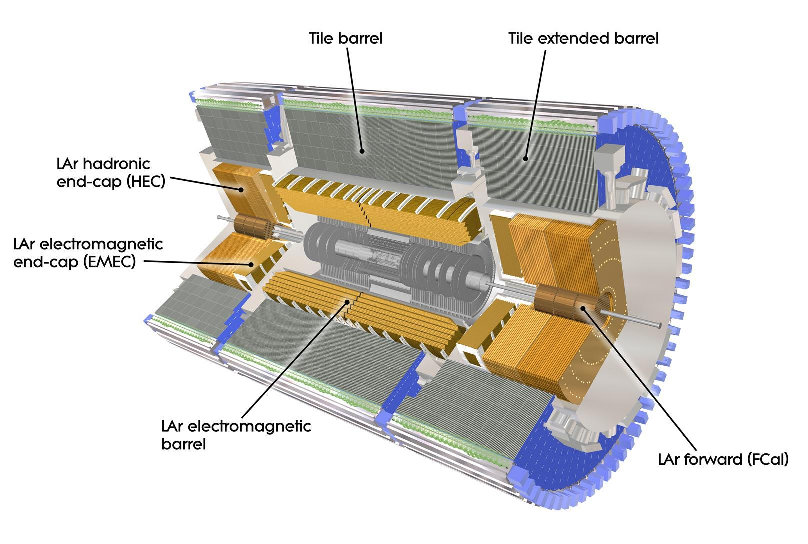
\includegraphics[width=0.9\textwidth]{Fig2/Calorimeters.pdf}
    \caption{Layout of the ATLAS electromagnetic and hadronic calorimeter systems. The total length is $\sim$ 12~m, extending to a maximum radius of 4.25~m.}
    \label{fig:figcalo}
  \end{center}
\end{figure}


\subsubsection{Liquid argon EM calorimeter}
  
The EM calorimeter uses lead as the absorber and liquid Argon as the active material. A photon traversing the absorber will interact with the heavy nucleus via Compton scattering or the photo-electric effect, producing low-energy electrons, or pair production, producing electron/positron pairs. An electron or positron, in turn, can produce bremsstrahlung photons as it is deflected by the nuclei or produce more charged particles via ionization. Thus each incident photon, electron, or positron produces a shower of photons, electrons, and positrons that lose their energy through successive interactions in the absorber. The produced particles ionize the liquid argon, and the charge is collected by electrodes located in the liquid argon gap.  These electrodes consist of three layers of copper sheets, the outer two kept at high-voltage potential and the inner one used to readout the signal.

To provide full coverage in $\phi$ without any cracks, an accordion-shaped absorber and electrode geometry is used, shown in Fig.~\ref{fig:EMacordion}.  This design was chosen to ensure high azimuthal uniformity, a regular liquid argon ionization gap, and a constant sampling fraction within a given detector region. The figure highlights  how this geometry is divided among rectangular cells in $\eta \times \phi$ space, the individual readout elements of varying size,  finely segmented both laterally and longitudinally. Such fine segmentation $– \Delta \eta \times \Delta \phi = 0.025 \times 0.025$ in the second layer of the EM barrel, for example $–$ permits a detailed mapping of the electromagnetic and hadronic showers. 

The position resolution of the EM is driven by the readout geometry (rectangular cells). There are three layers of cells, segmented along the particle's direction of motion.  The $\phi$ segmentation comes from grouping the accordion-shaped electrodes together into a common read out channel. 

In the region $0 <|\eta| < 1.8$ the electromagnetic calorimeters are complemented by a ``presampler'' detector, an instrumented argon layer, which provides a measurement of the energy lost in the solenoid and the outer wall of the barrel cryostat.

The signal readout chain for the LAr calorimeter (indeed for all calorimeter systems) is divided into a fast analog readout for the trigger system and a slower digital readout used for more redefined trigger decisions and the offline reconstruction. However, regardless of the readout path, the signal is initiated within the active LAr medium.  Shaping electronics induce a bipolar puse shape in the ionization signal. This shape is characterized by having both a positive and a negative component, which renders the integral of the signal exactly equal to zero.

The performance of the shaping electronics is critical for a correct energy calibration of the detector since the energy is primarily determined from the peak height of the pulse. % Figure??
In each calorimeter region, the overall pulse shape and duration are optimized to approximately cancel a constant injection of energy into the detector. The motivation for this approach is to effectively redefine the baseline of the energy measurement. In the high luminosity environment of the LHC, this reduces the sensitivity to the background from multiple $pp$ interactions on average.

Finally, the EMEC uses the same accrodion geometry as the EMB, whereas the granularity is typically slightly larger than in the barrel.

 %The first sampling layer has a depth of 4.3$X_0$\footnote{$X_{0}$ es el s\'imbolo utilizado para la Longitud de Radiaci\'on (\emph{Radiation length}), definida como la distancia media sobre la cual un elect\'on muy energ\'etico pierde $1/e$ de su energ\'ia por bremsstrahlung o bien, como $7/9$ del camino libre medio en la producci\'on de pares. Contituye una escala de longitud apropiada para describir cascadas electromagn\'eticas de alta energ\'ia.}
%Towers of readout cells with coarser granularity, $0.1 \times 0.1$ in the barrel, sum the energy in all three layers of cells and feed information to the trigger system.

\begin{figure}[htbp]
  \begin{center}
      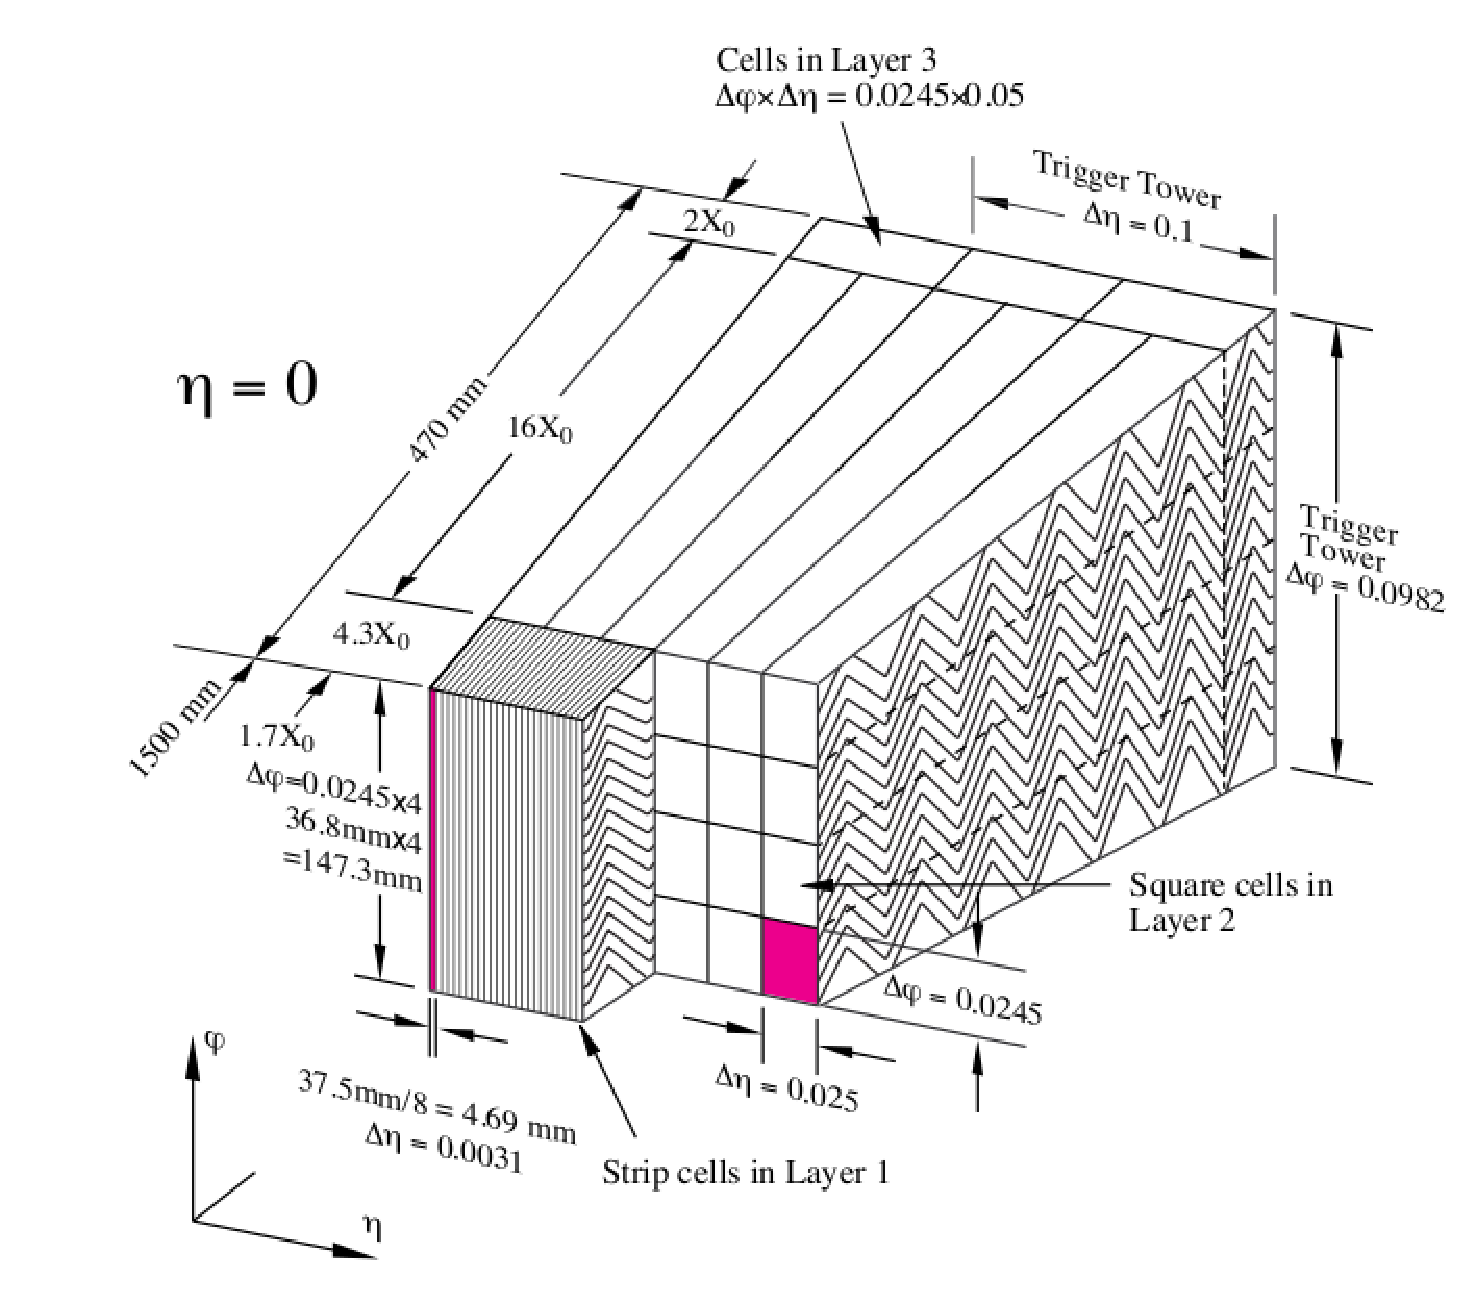
\includegraphics[width=0.9\textwidth]{Fig2/EM_acordionstructure.pdf}
    \caption{Cross section of the LAr barrel calorimeter where the different layers are visible. The granurality in $\eta$ and $\phi$ of the cells of each of the three layers is also shown.}
    \label{fig:EMacordion}
  \end{center}
\end{figure}



\subsubsection{The hadronic calorimeter}
% TileCal [ ] Tile Calorimeter Technical Design Report, CERN/LHCC 96-42, 15-12-1996;


Outside the EM calorimeter lies the system of hadronic calorimeters. The barrel portion, known as the Tile calorimeter, uses iron absorber slabs interspersed with scintillating tiles. The Tile calorimeter is most notable for its depth of 7.4 radiation lengths ($\lambda$\footnote{To quantify the amount of material needed to capture a particles's energy, the unit of an interaction length, which is the distance over which a high energy charged particle loses $1-\frac{1}{e}\sim 63$\% of its energy , is commonly used.}). The hadronic end-cap and the forward calorimeter, which need to absorb the more energetic particles that are produced at large $|\eta|$, are made of copper and tungsten abosrbers, respectively, with liquid argon as the active material.

The tile calorimeter is composed of 3~mm thick scintillating tiles, arranged to lie parallel  to the incoming particle direction, interleaved with 14~mm thick iron plates. %as shown in Figure!!!!!!!!!!!
It is divided into the barrel calorimeter, covering $|\eta|<1.0$, and two extended barrel calorimeters, covering  $0.8 < |\eta| <1.7$. Each tile is read out by two wavelength-shifting fibers, which convert the scintillator signal to visible light. The readout fibers of several tiles are grouped to a single photomultiplier tube forming cells in $\eta \times \phi$ space. As in the EM calorimeter, these cells are segmented into three layers, the first two of size $\Delta \eta = 0.1$ and  $\Delta \phi = 0.1$ and the last of size   $\Delta \eta = 0.2$ and  $\Delta \phi = 0.1$.  Towers to provide information to the trigger systema are formed from 0.1$\times$0.1 grouping of all three layers.



%------------------------------------------------------------------------
\subsection{The Muon System}\label{sec:atlasCALO}
%------------------------------------------------------------------------
 El sistema de muones sirve a un doble prop\'osito: funciona como sistema de disparo (o \emph{trigger}) para la selecci\'on de eventos con muones de alta energ\'ia, y como espectr\'ometro de muones de alta precisi\'on. En este sentido, este detector llevar\'a a cabo la identificaci\'on de los muones producidos en las colisiones \emph{p-p}, determinando sus trayectorias y momentos.
% Las part\'iculas provenientes del punto de interacci\'on atraviesan tres conjuntos de c\'amaras, uno situado previo al toroide, uno interior y otro posterior. 
   El sistema consiste en un conjunto de toroides (llamamos as\'i, por su forma, a los tres conjuntos de bobinas que proveen el campo magn\'etico toroidal) y c\'amaras de tubos de deriva que se encuentran rodeando al calor\'imetro. En la parte del barril del detector, las c\'amaras est\'an situadas en el interior del toroide lo que permite la medici\'on del momento de las part\'iculas a partir de la desviaci\'on de sus trayectorias en el campo magn\'etico. En las tapas, donde la presencia del cri\'ostato impide posicionar las c\'amaras dentro del campo magn\'etico, el momento es medido a partir de la diferencia entre los \'angulos de entrada y salida del im\'an.
En el plano trasversal, tanto en la regi\'on del barril como en las tapas laterales, el sistema de c\'amaras estar\'a dividido en 16 sectores, siguiendo la simetr\'ia determinada por las 8 bobinas del barril central del sistema magn\'etico. Las c\'amaras cubren el espacio entre las bobinas, y todo el rango acimutal en la regi\'on que las rodea. Los sectores se numeran comenzando a partir de $\phi = 0$, en el sentido contrario de las agujas del reloj, teniendo en la direcci\'on vertical a los sectores 6 (en la parte superior del detector) y 13 (sector inferior).  

   Los c\'amaras de tubos de deriva (MDTs) son c\'amaras proporcionales hechas de tubos de aluminio de 30 mm de di\'ametro y longitudes variables de 70 a 630 cm, con un hilo central de 50$\mu$m de di\'ametro, de W-Re. En la regi\'on del barril dichas c\'amaras est\'an distribuidas en 3 capas cil\'indricas conc\'entricas (estaciones) alrededor del haz, de 5; 7,5 y 10 metros de radio. Los tubos est\'an dispuestos de manera transversal al eje \emph{z} de manera de medir la coordenada en el plano de desviaci\'on de la trayectoria de la part\'icula (plano \emph{Rz}).  Estas c\'amaras miden el tiempo de deriva de la ionizaci\'on producida por el paso del mu\'on, teniendo una resoluci\'on de 80 $\mu$m.
% MAS del TDR? Falta los radios de las estaciones(?)
   
   Cada c\'amara MDT est\'a cubierta por una o dos c\'amaras de placas resistivas (RPCs). Cada una de ellas encierra un volumen de gas entre planchas resistivas de baquelita, dotada una de ellas con tiras de electrodos. Dado que los tubos de deriva poseen un di\'ametro relativamente grande que resulta en un tiempo de deriva m\'aximo de 480ns, mucho mayor que los 25 ns entre cruce de \emph{bunches}, se requieren c\'amaras especiales de disparo para la selecci\'on de eventos. La funci\'on de trigger en el barril es provista por tres capas de RPCs, situadas, dos de ellas, a ambos lados de la segunda estaci\'on de MDTs y la restante, en la cara interior de la estaci\'on m\'as externa. 
En las tapas, esta funci\'on es cumplida por tres estaciones de TGCs (\emph{Thing Gap Chambers}). Estas c\'amaras son similares en dise\~no a c\'amaras prporcionales multihilo, con la diferencia de que poseen una distancia c\'atodo-c\'atodo menor que la pendiente del \'anodo (hilo). 
   Las c\'amaras de disparo proveen una estimaci\'on de las coordenadas $\phi$ y $\eta$ del punto de impacto de la traza, mientras que las c\'amaras MDTs dar\'an (con mayor precisi\'on) la coordenada $\eta$.

    En la regi\'on de bajo \'angulo, donde la densidad de trazas es mayor, se utilizan c\'amaras de tiras de c\'atodos (CSCs) de granularidad m\'as fina comparadas con las MDTs, para la detecci\'on de trayectorias. Estas c\'amaras son c\'amaras proporcionales, con un espacio entre hilo de 2,5 mm. Cada una de ellas proporciona medida de dos coordenadas y puede operar en condiciones de alto campo magn\'etico.

   En la figura \ref{fig:MUON1} se puede ver un esquema del espectr\'ometro de muones, donde se indica la posici \'on de las diferentes c\'amaras descriptas.

\begin{figure}[htbp]
  \begin{center}
      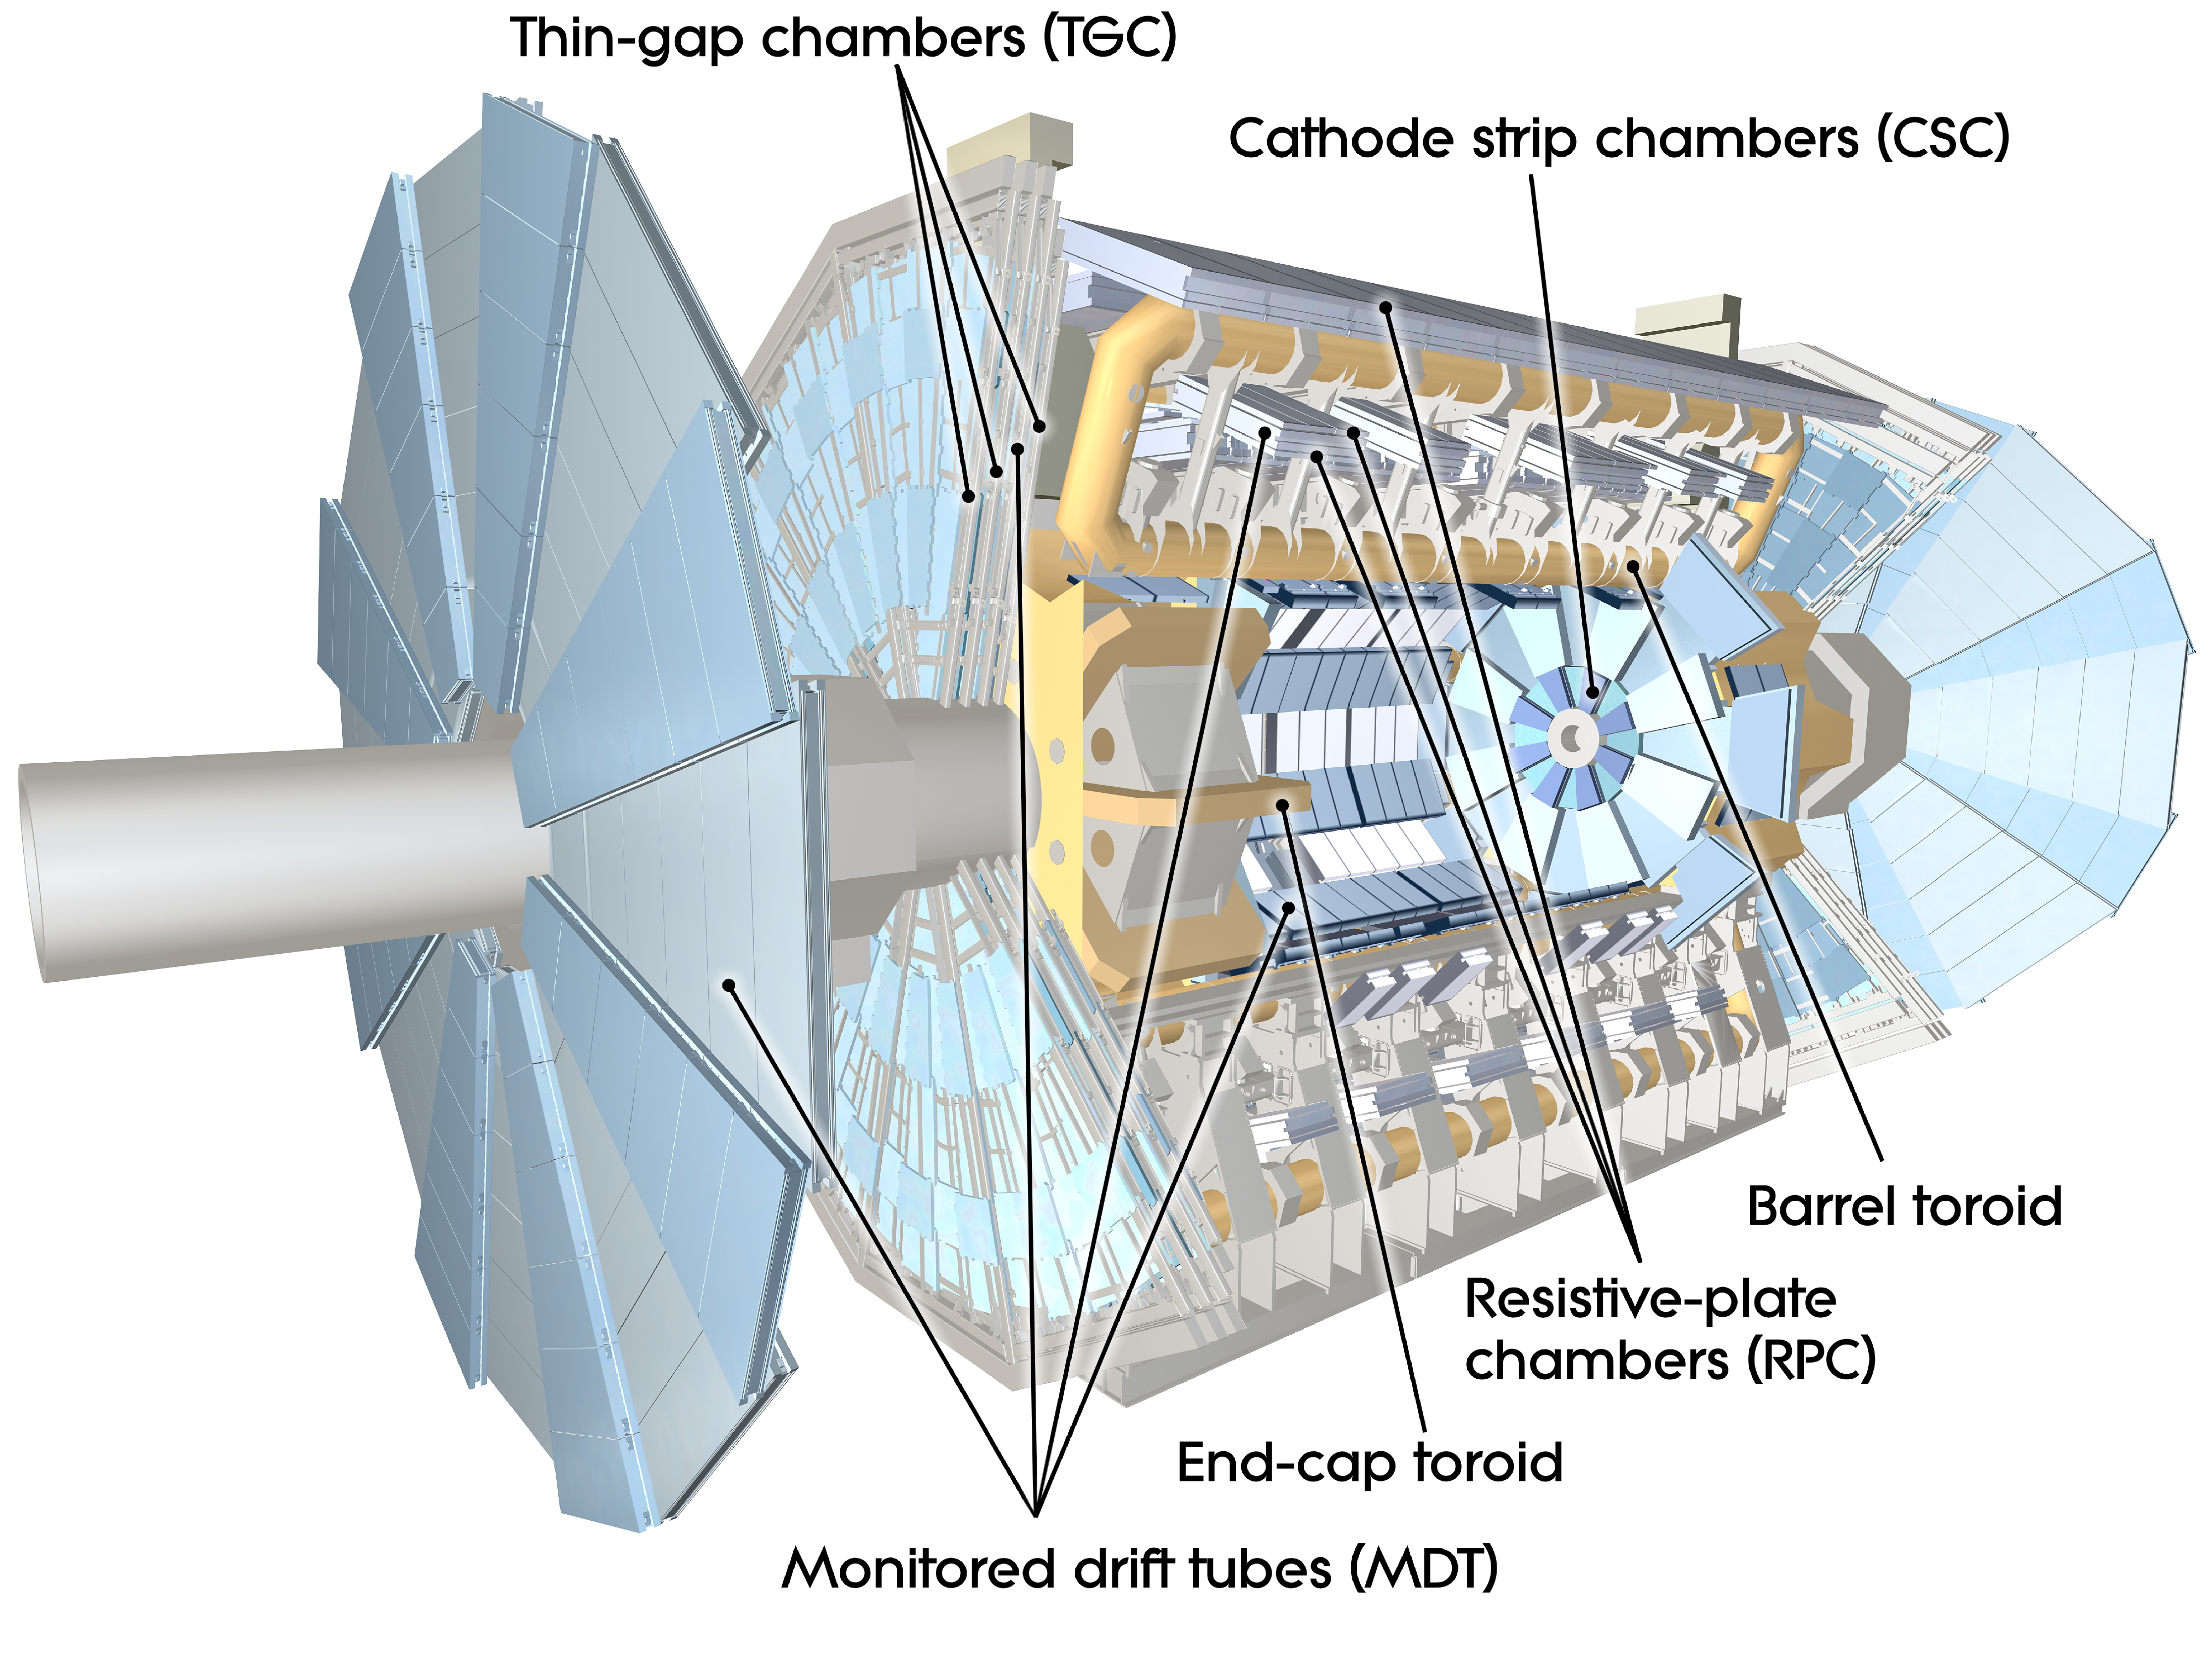
\includegraphics[width=0.8\textwidth]{Fig2/MuonChamber.pdf}
    \caption{Muon Chamber}
    \label{fig:MUON1}
  \end{center}
\end{figure}



%EL SYSTEMA DE IMANES!!!!!!!!!!!!!!!!!!!!!!!!!!!!!!!!!!!!!!!!!!!!!!!!!!!!!!!!!!!!!!!!

El sistema de imanes superconductores de ATLAS consiste en un solenoide central que provee el campo magn\'etico necesario al detector interno, rodeado por un arreglo de bobinas o bucles, con forma de pista de carrera, que generan un campo magn\'etico toroidal para el espectr\'ometro de muones.Todo el sistema es enfriado de manera indirecta mediante el flujo de helio l\'iquido a 4,5 K.

   El solenoide es un electroim\'an superconductor de 5,3 m de largo, situado en el interior del calor\'imetro electromagn\'etico. Comparte el cri\'ostato con el calor\'imetro de arg\'on l\'iquido, evitando la presencia de dos paredes criost\'aticas y reduciendo as\'i la cantidad de material introducido. La longitud del solenoide es considerablemente m\'as peque\~na que la del barril del detector de trazas. Este es el resultado de un compromiso: un bobinado corto reduce la cantidad de material introducido mientras que uno largo proporciona un campo magn\'etico m\'as uniforme en dicho detector. El campo magn\'etico a lo largo del eje \emph{z} es de 2 T en el punto de interacci\'on.
% existe .criost\'aticas.?

   El arreglo de bobinas est\'a dividido en un barril central y dos regiones laterales, al igual que los detectores. El barril central est\'a constituido por 8 bobinas de 5 m de ancho por 25 metros de largo aproximadamente, dispuestas sim\'etricamente alrededor del haz de manera radial. Las bobinas del barril se encuentran en cri\'ostatos separdos, mientras que las 8 bobinas en cada una de las tapas o toroides laterales est\'an ubicadas en un cri\'ostato com\'un.

   Con un campo magn\'etico toroidal las part\'iculas atravesar\'an todo el rango de pseudorapidez casi perpendicularmente al haz. El n\'umero peque\~no de bobinas que generan el campo toroidal resulta en una intensidad de campo que var\'ia fuertemente con la coordenada $\phi$. En el barril el campo magn\'etico es de 2 T, mientras que en las tapas es de 4 T en las zonas de mayor intensidad.   



%------------------------------------------------------------------------
\subsection{Trigger and Data Adquisition}\label{sec:atlasCALO}
%------------------------------------------------------------------------
 En este cap\'itulo se analiza la estructura del trigger de ATLAS, y el sistema de adquisici\'on y flujo de los datos. Se presenta, asimismo, una breve descripci\'on de los algoritmos usados en la reconstrucci\'on de trayectorias para la selecci\'on de eventos en el detector interno. 


\subsubsection{Arquitectura general}

   El sistema de Trigger y Adquisici\'on de Datos\cite{TDRtdaq} de ATLAS est\'a basado en tres niveles de selecci\'on \emph{online}: Nivel 1, Nivel 2 y Filtro de Eventos. Cada nivel es m\'as lento pero m\'as preciso que el anterior. Trabajando con una frecuencia de interacci\'on de $10^{9}$ Hz y luminosidades del orden de $10^{34}$ $cm^{-2}$ $s^{-1}$, este sistema ser\'a el encargado de reducir la frecuencia de eventos inicial de 40 MHz a 200Hz, que es la velocidad con la que pueden almacenarse. 

   En la figura \ref{fig:TDAQ} se muestra un vista simplificada de los principales componentes y funciones.  

\begin{figure}[!h]
\begin{center}
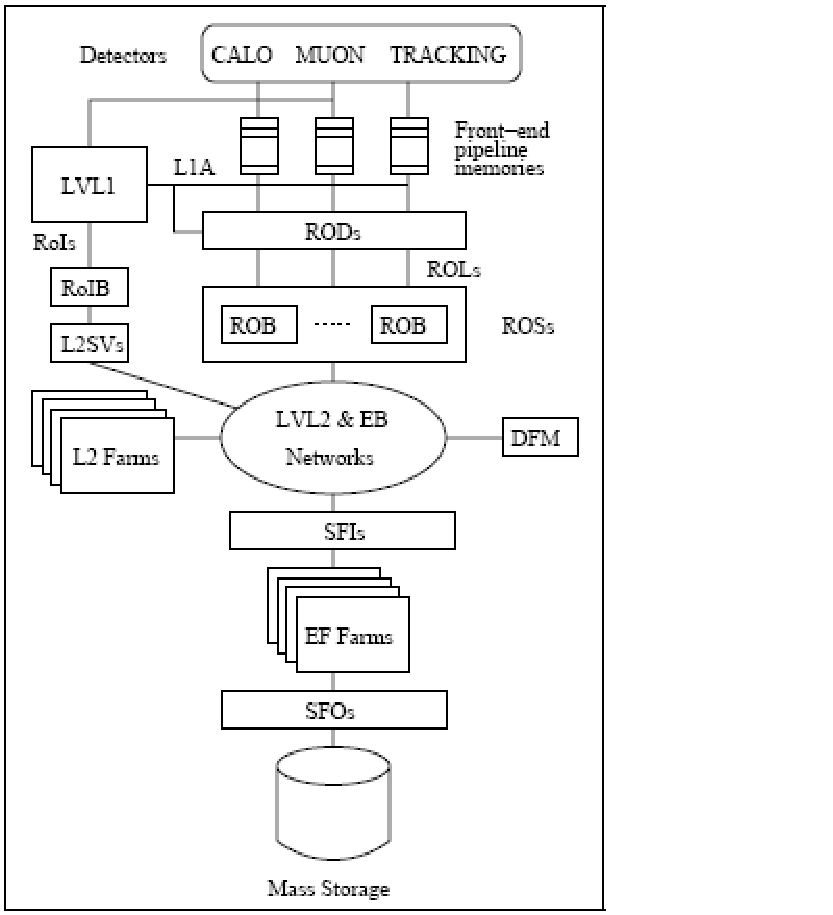
\includegraphics[width=0.5\textwidth]{Fig3/paint_TDAQ.pdf}
\caption{Principales componentes del sistema de trigger y adquisici\'on de datos de ATLAS. } 
\label{fig:TDAQ}
\end{center}
\end{figure}

   El mecanismo que lleva a cabo el movimiento de la informaci\'on (Data Flow System), es el responsable de recibir los datos de los detectores, pasando parte de ellos al sistema de trigger y enviando luego, los eventos seleccionados al lugar de almacenamiento. Siguiendo el esquema de la figura, la comunicaci\'on entre los \emph{drivers} de lectura %controladores de lectura?
de cada detector (RODs) y el sistema de adquisici\'on de datos, est\'a dada por los \emph{buffers} de almacenamiento transitorio (ROBs). La informaci\'on de los eventos aceptados por el Nivel 1 son transportados de los primeros al sistema de lectura (ROS), que consta de numerosos ROBs, guardando los datos a la espera de la decisi\'on del trigger. La informaci\'on requerida por el segundo nivel es provista por estos \'ultimos. Los eventos aceptados son reconstruidos (a partir de fragmentos contenidos en diferentes ROBs) y pasados al siguiente nivel.
%(\emph{Read Out Drivers})
%(\emph{Read Out Buffers})
% (\emph{Read Out System})

   El Nivel 2 y el Filtro de Eventos componen el \emph{High-level Trigger} (HLT) de ATLAS. El Nivel 2 trabaja a la frecuencia de aceptaci\'on del Nivel 1, utilizando una secuencia de r\'apidos algoritmos de selecci\'on que operan t\'ipicamente sobre una fracci\'on de los datos del evento, contenida en regiones del detector previamente seleccionadas por ese nivel (ver el mecanismo de la regi\'on de inter\'es en la siguiente secci\'on). Si la decisi\'on del Nivel 2 es rechazar el evento, los datos del mismo son eliminados de los buffers correspondientes. Si el evento es aceptado,  se reconstruye  en el EB (Event Builder) y es pasado al Filtro de Eventos. Este nivel ejecutar\'a algoritmos de reconstrucci\'on m\'as sofisticados, adaptados de aquellos para el an\'alisis \emph{offline}, utilizando informaci\'on detallada de los detectores para efectuar el proceso de selecci\'on final, que determinar\'a cu\'ales son los eventos que ser\'an guardados para posteriores estudios.

  En las siguientes secciones se presenta una descripci\'on m\'as detallada de los niveles de trigger.

 
\subsubsection{El Nivel 1}

   El primer nivel de trigger de ATLAS es implementado mediante hardware. \'Este realiza una decisi\'on inicial a partir de la informaci\'on provista por los calor\'imetros y del detector de muones, basando su estrategia en la combinaci\'on de objetos en coincidencia. %or veto.
  
   En el sistema de muones, los candidatos de alto momento transverso son identificados en las c\'amaras especiales de trigger: RPCs en el barril y TGCs en las tapas. En el caso del calor\'imetro, se definen una serie de conjuntos de umbrales de $p_T$ para cada objeto (electrones, fotones, jets, etc.), seleccionando aquellos que pasen los criterios de selecci\'on correspondientes al evento f\'isico de inter\'es. 

   Puesto que la decisi\'on de aceptar un evento no puede ser realizada en los 25 ns que median entre dos cruces de \emph{bunches}, los subdetectores almacenan localmente la informaci\'on del mismo en \emph{pipelined buffers} hasta que el Nivel 1 efect\'ua la selecci\'on. Luego, los datos son enviados a los RODs especi\'ficos de cada detector para luego dirigirse a los ROBs, donde son almacenados hasta que la decisi\'on del Nivel 2 sea alcanzada. 
   Cuando un evento es aceptado, el Nivel 1 comunica la decisi\'on al mecanismo que se encargar\'a de construir una Regi\'on de Inter\'es (RoI). Este mecanismo es una importante pieza sobre la que descansa la estrategia del sistema de trigger; a trav\'es del mismo, el Nivel 2 har\'a uso de la informaci\'on del evento en regiones localizadas del detector, de manera que los algoritmos de reconstrucci\'on en ese nivel s\'olo transfieran los ROBs necesarios para arribar a una r\'apida decisi\'on. %Es importante notar que la informaci\'on de todos los subdetectores est\'a disponible para dichos algoritmos en caso de ser necesario.
La RoI contendr\'a la informaci\'on de la posici\'on ($\eta$ y $\phi$) y el momento de los objetos candidatos.

   Este nivel est\'a dise\~nado para llevar a cabo su decisi\'on en un tiempo menor a 2.5 $\mu$s, medidos desde la colisi\'on \emph{p-p}, hasta que la informaci\'on del evento est\'a disponible en la electr\'onica de salida de los detectores. En este proceso la frecuencia de eventos ser\'a reducida a 75KHz (l\'imite fijado por la electr\'onica).

\subsection{El HLT}

 El High-level Trigger de ATLAS abarca la segunda y tercera etapa de la selecci\'on de eventos. Comprende el Nivel 2 y el Filtro de Eventos, y contiene adem\'as, el Software de Selecci\'on (ESS). Este \'ultimo comparte la estructura usada por el Offline para los c\'odigos de selecci\'on, facilitando el an\'alisis \emph{offline} de los datos, y el desarrollo de algoritmos en el HLT.

   El punto de entrada del trigger es el resultado del Nivel 1. \'Este provee informaci\'on acerca de la regi\'on de inter\'es, fundamental para el r\'apido funcionamiento de los algoritmos del Nivel 2. As\'i, los datos del Nivel 1 gu\'ian la selecci\'on del Nivel 2; y \'esta a su vez guiar\'a la del Filtro de eventos, como se ilustra en la figura \ref{fig:HLTchainseed}. 
%HLTchain_seeding.pdf
\begin{figure}[!h]
\begin{center}
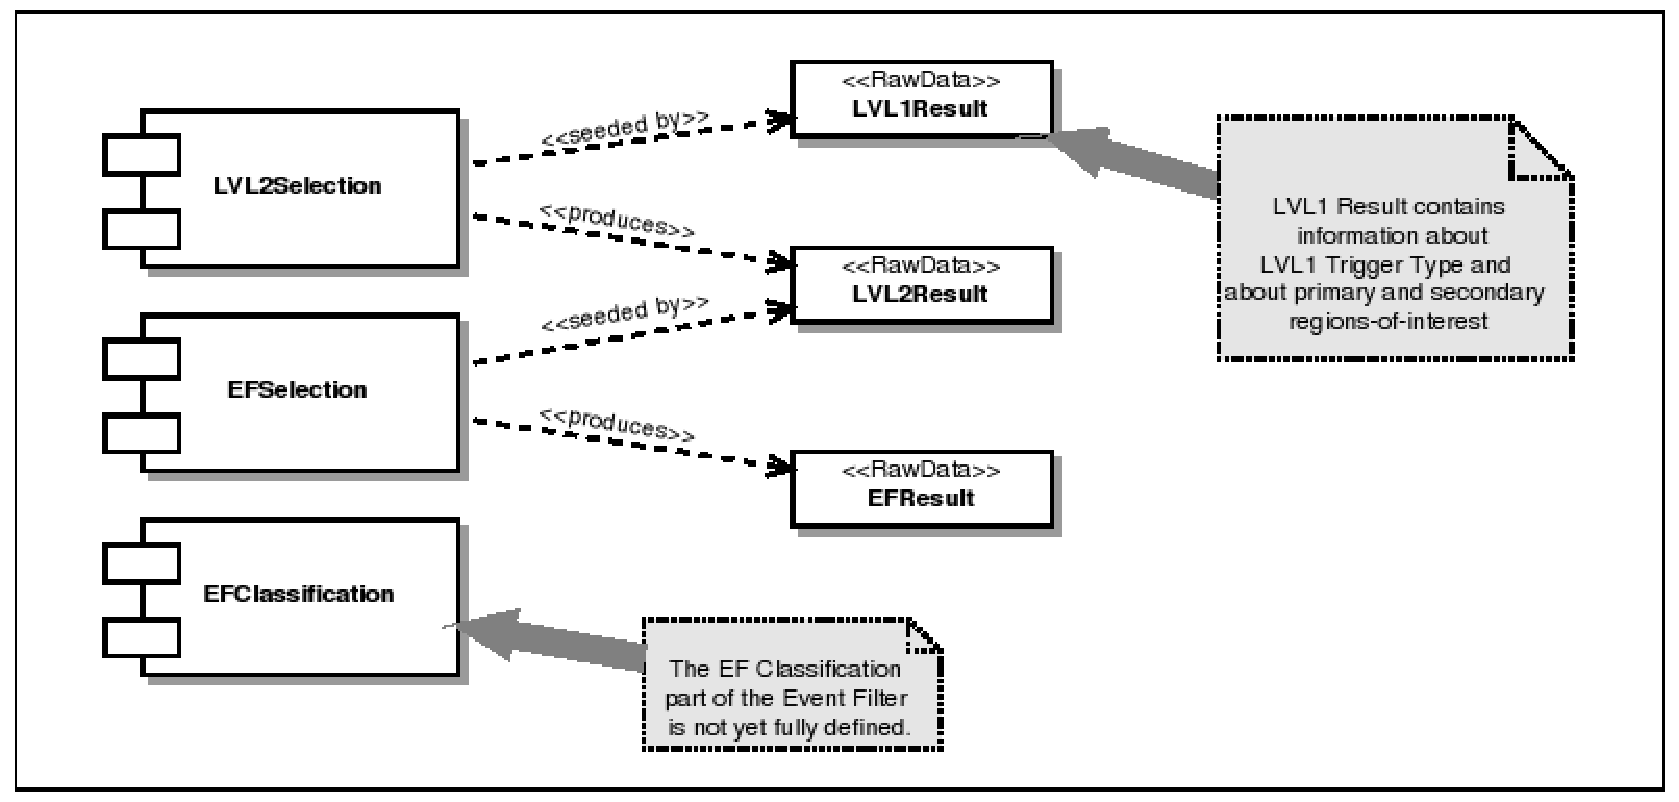
\includegraphics[width=0.9\textwidth]{Fig3/HLTchain_seeding.pdf} 
\caption{Cadena de selecci\'on del \emph{High-level Trigger} de ATLAS. Cada nivel es guiado por el resultado del paso anterior.}
\label{fig:HLTchainseed}
\end{center}
\end{figure}


\subsubsection{El Nivel 2}
   La tarea espec\'ifica del Nivel 2 es reducir la frecuencia de eventos de $\sim$ 100 kHz a alrededor de 2 kHz, combinando la informaci\'on de todos los detectores para su decisi\'on global. A diferencia del Nivel 1, esta segunda etapa de selecci\'on realiza operaciones no sincronizadas sobre los eventos, con un tiempo de decisi\'on de 10 ms.
%asynchronous??

   El Nivel 2 utiliza las regiones de inter\'es provistas por el Nivel 1. Cada regi\'on es examinada en el subdetector de origen (calor\'imetro o sistema de muones) para su confirmaci\'on; para luego buscar informaci\'on de otros subdetectores. En el caso del trigger de muones, el poder de rechazo del Nivel 2 proviene de ajustar los umbrales de $p_{T}$, respecto de los utilizados en el primer nivel, a partir de la informaci\'on de las c\'amaras de precisi\'on del sistema de muones (MDTs) y la correspondiente al detector interno.
Los procesadores del Nivel 2 son los encargados de ejecutar luego el software de selecci\'on de eventos, utilizando la informaci\'on almacenada en los \emph{buffers}. Usando las RoIs del Nivel 1, el Nivel 2 acceder\'a de manera selectiva a los datos en los ROBs, moviendo s\'olo la informaci\'on requerida para efectuar la decisi\'on. T\'ipicamente, s\'olo una peque\~na fracci\'on del detector, correspondiente a las regiones centradas en los objetos indicados por el Nivel 1, ser\'an necesitados por el segundo nivel.

  Hasta que un evento es aceptado o rechazado (en $\sim$ 10 ms), los datos son retenidos en los ROBs. En caso de aceptaci\'on, los fragmentos del evento almacenados en distintos buffers ser\'an requeridos por el sistema de control del Nivel 2 (L2SVs) para ser enviados al constructor de eventos (EB). El evento ensamblado es guardado en una \'unica direcci\'on de memoria para ser utilizado por el Filtro de Eventos. El tama\~no promedio de un evento ser\'a del orden de 1,5 MB.


\subsubsection{El Filtro de Eventos}

  Luego del Nivel 2, la \'ultima etapa de selecci\'on \emph{online} es realizada por el Filtro de Eventos (EF). El EF emplea algoritmos y m\'etodos similares a los implementados en el an\'alisis \emph{offline}, adaptados para su corrida en el tiempo real del experimento; su poder de rechazo radica en el uso de algoritmos y criterios de selecci\'on m\'as complejos, que por l\'imites en el tiempo de procesamiento no pueden ser utilizados en el Nivel 2.
  
  El EF utilizar\'a informaci\'on actualizada de la calibraci\'on y alineamiento del detector y un completo mapa del campo magn\'etico; llevando a cabo con ello la selecci\'on final del evento f\'isico que ser\'a guardado para su estudio en el Offline. La frecuencia de aceptaci\'on del nivel anterior ser\'a reducida en un orden de magnitud, almacenando a una tasa de $\sim$100 MB/s.


\subsubsection{El software de selecci\'on}
\label{'HLTalgos'}
   
 La tarea del software de selecci\'on (ESS) es la selecci\'on y clasificaci\'on de los eventos. Candidatos tales como electrones, jets, muones, etc., representados por objetos abstractos, son reconstruidos utilizando un particular conjunto de algoritmos. Un evento es seleccionado si el objeto reconstruido satisface al menos una de las signaturas establecidas en el men\'u del sistema de disparo. En el Nivel 2 y el Filtro de Eventos (EF), los eventos ser\'an rechazados si no pasan los espec\'ificos criterios de selecci\'on, dise\~nados para la reducci\'on de la frecuencia de eventos, al l\'imite dado por la velocidad a la que \'estos pueden ser almacenados.

 El ESS se compone de una infraestructura y un conjunto de programas de selecci\'on para las dos etapas del HLT.  Los algoritmos de reconstrucci\'on para el trigger est\'an basados en aquellos utilizados para la reconstrucci\'on \emph{offline}, pero correr\'an \emph{online} en el entorno de software provisto por los procesadores del Nivel 2 y el EF. 

  De manera de facilitar el desarrollo de los algoritmos del HLT y simplificar los estudios del Offline; el ESS ha sido dise\~nado de manera de poder ser ejecutado directamente en el entorno provisto por la estructura de software de an\'alisis offline del experimento, ATHENA\cite{Athena}. La estructura dada por este paquete de software es lo suficientemente flexible como para abarcar una variedad de procesos, incluyendo no s\'olo algoritmos de trigger sino tambi\'en tareas de calibraci\'on y monitoreo. Se ha destinado un ap\'endice (A) para su descripci\'on.
 
  En el Offline, la tarea del ESS es la de emular la cadena completa de selecci\'on \emph{online}. Para su ejecuci\'on el sistema se sirve de cuatro sub-paquetes: el direccionamiento o \emph{Steering}, los algoritmos del HLT, y los paquetes de software para la clasificaci\'on y movimiento de los datos, EDM (\emph{Event Data Model}) y el DM (\emph{Data Manager}). Los \'ultimos toman los datos del evento en el formato que poseen a la salida de los sistemas de lectura (\emph{Raw data} en formato \emph{byte stream}), y los convierten en objetos que puedan ser usados por los algoritmos en la cadena de selecci\'on (\emph{Raw Data Objects}).

  La tarea de los algoritmos del HLT es la de analizar los datos del evento, reconstruyendo partes del mismo, luego de la selecci\'on del Nivel 1. El paquete se compone de dos subconjuntos principales:
%itemize
\begin{itemize}
   \item Programas de preparaci\'on de datos. Son los algoritmos ejecutados por los sistemas EDM y DM para la conversi\'on del formato de los datos del evento. 
   \item Algoritmos FEX o de \emph{Feature Extraction}. Comprende los programas de reconstrucci\'on y los llamados algoritmos de ``hip\'otesis''. Estos \'ultimos (a los primeros nos referiremos en la siguiente secci\'on) son aquellos programas que se encargan de eliminar, una vez realizada la reconstrucci\'on, aquellos candidatos que no cumplen con las caracter\'isticas o atributos asignados al evento f\'isico en consideraci\'on (hip\'otesis), aplicando espec\'ificos criterios de selecci\'on. La presencia de los algoritmos de hip\'otesis es fundamental en la secuencia del HLT ya que evita la ejecuci\'on innecesaria de algoritmos al descartar eventos en las primeras etapas de la cadena.
\end{itemize}

  Por \'ultimo, el subpaquete de \emph{Steering} es aquel que organiza el procesamiento de los datos del evento en el Nivel 2 y el Filtro de eventos; controlando el orden en el que los algoritmos de reconstrucci\'on e hip\'otesis son ejecutados. El Steering define la secuencia del HLT, y manipula los resultados en cada paso de selecci\'on de manera que la decisi\'on del trigger sea alcanzada.


%------------------------------------------------------------------------
\subsection{Data quality}\label{sec:atlasSim}
%------------------------------------------------------------------------

%------------------------------------------------------------------------
\subsection{Simulation of particle interactions in the ATLAS Detector}\label{sec:atlasSim}
%------------------------------------------------------------------------



